\documentclass[a4paper,9pt,journal,twoside,compsoc]{PPIEEEtran}

% In the ReportType command chose "act" for Activity Report or "learn" for Learnings Report
\newcommand*{\ReportType}{}

% -----------------------------------------------------------------------------
% The Preamble document contains all the necessary Packages for typesetting
% Modify it to suit your needs
% -----------------------------------------------------------------------------

%%%%%%%%%%%%%%%%%%%%%%%%%%%%%%%%%%%%%%%%%%%%%%%%%%%%%%%%%%%%%%%%%%%%%%%%%%%%%%%%
%2345678901234567890123456789012345678901234567890123456789012345678901234567890
%        1         2         3         4         5         6         7         8
% Required Packages and commands
% --> Please Choose the MAIN LANGUAGE for the document in package BABEL (below)
% --> Please Choose the TYPE OF REPORT for the document in \ReportType (below)
% !TEX root = ./main.tex
% PP_Report_Preamble.tex
% V2.1
% 2017/05/07
% by Rui Santos Cruz
%%%%%%%%%%%%%%%%%%%%%%%%%%%%%%%%%%%%%%%%%%%%%%%%%%%%%%%%%%%%%%%%%%%%%%%%%%%%%%%%
%
% *** INPUT LANGUAGE PACKAGES ***
% Choose the main language in package Babel
\usepackage[main=english]{babel}
\usepackage[utf8]{inputenc}
\usepackage{iflang}

\usepackage{dsfont}
\newcommand*{\Z}{\mathds{Z}}
\newcommand*{\R}{\mathds{R}}

% *** ACRONYM PACKAGES ***
% Put definition of Acronyms at the end of the document
\usepackage[printonlyused,nolist]{acronym}

% *** CITATION PACKAGES ***
\usepackage{cite}

% *** GRAPHICS RELATED PACKAGES ***
\usepackage[pdftex]{graphicx}
\graphicspath{ {images/} }
\DeclareGraphicsExtensions{.pdf,.jpeg,.png}

% *** MATH PACKAGES ***
\usepackage[cmex10]{amsmath}

% *** SPECIALIZED LIST PACKAGES ***
\usepackage{algorithmic}

% *** ALIGNMENT PACKAGES ***
\usepackage{array}

% *** SUBFIGURE PACKAGES ***
\usepackage[caption=false,font=normalsize,labelfont=sf,textfont=sf]{subfig}

% *** FLOAT PACKAGES ***
\usepackage{fixltx2e}

% *** PDF, URL AND HYPERLINK PACKAGES ***
\usepackage{url}

% *** CODE PACKAGES ***
\usepackage{listings}


% *** BACKGROUND Material ***
\usepackage{eso-pic}
\usepackage[
  contents={},
  opacity=1,
  scale=1,
  color=blue!90
  ]{background}
  
% *** CONDITIONALS ***
\usepackage{ifthen}

% Clever Referencing
% Note: portuguese is supported through "brazilian" option
\usepackage[\IfLanguageName{english}{english}{brazilian}]{cleveref}

%%%%%%%%%%%%%%%%%%%%%%%%%%%%%%%%%%%%%%%%%%%%%%%%%%%%%%%%%%%%%%%%%%%%%%%%%%%%%%%%
% PLEASE DO NOT CHANGE THIS SECTION
% Printing the Scoring Table
%%%%%%%%%%%%%%%%%%%%%%%%%%%%%%%%%%%%%%%%%%%%%%%%%%%%%%%%%%%%%%%%%%%%%%%%%%%%%%%%

\begin{document}
% correct bad hyphenation here
\hyphenation{op-tical net-works semi-conduc-tor}
%%%%%%%%%%%%%%%%%%%%%%%%%%%%%%%%%%%%%%%%%%%%%%%%%%%%%%%%%%%%%%%%%%%%%%%%%%%%%%%%


%%%%%%%%%%%%%%%%%%%%%%%%%%%%%%%%%%%%%%%%%%%%%%%%%%%%%%%%%%%%%%%%%%%%%%%%%%%%%%%%
%% PP_Report_Cover.tex
%%%%%%%%%%%%%%%%%%%%%%%%%%%%%%%%%%%%%%%%%%%%%%%%%%%%%%%%%%%%%%%%%%%%%%%%%%%%%%%%
% paper title
% can use linebreaks \\ within to get better formatting as desired
% Do not put math or special symbols in the title.
\title{Active Debris Removal:\\Ant Colony System algorithms for Dynamic TSP}

%%%%%%%%%%%%%%%%%%%%%%%%%%%%%%%%%%%%%%%%%%%%%%%%%%%%%%%%%%%%%%%%%%%%%%%%%%%%%%%%
% Author names
%
% note positions of commas and nonbreaking spaces ( ~ ) LaTeX will not break
% a structure at a ~ so this keeps an author's name from being broken across
% two lines.
% use \thanks{} to gain access to the first footnote area
% a separate \thanks must be used for each paragraph.
%
%\IEEEcompsocitemizethanks is a special \thanks that produces the bulleted
% lists for "first footnote" author affiliations. 
% Use \IEEEcompsocthanksitem which works much like \item
% for each affiliation group.
\author{Emanuele~Lovera - 901727 - University of Milan. %<-this % stops a space
% Change the Course Name 
% note: need leading \protect in front of \\ to get a newline within \thanks as
% \\ is fragile and will error, could use \hfil\break instead.
}

%%%%%%%%%%%%%%%%%%%%%%%%%%%%%%%%%%%%%%%%%%%%%%%%%%%%%%%%%%%%%%%%%%%%%%%%%%%%%%%%
% Prints in Subtitle the type of Report
% PLEASE DO NOT CHANGE THIS SECTION

%%%%%%%%%%%%%%%%%%%%%%%%%%%%%%%%%%%%%%%%%%%%%%%%%%%%%%%%%%%%%%%%%%%%%%%%%%%%%%%%
%%%%%%%%%%%%%%%%%%%%%%%%%%%%%%%%%%%%%%%%%%%%%%%%%%%%%%%%%%%%%%%%%%%%%%%%%%%%%%%%
% The paper Abstract and Keywords
\IEEEtitleabstractindextext{%

\begin{abstract}
The Active Debris Removal -- ADR -- is a growing threat for space operations in Low Earth Orbit. Some passive actions are made for limiting this phenomenon, but in the future will be necessary to actively remove satellite debris. An ADR Mission will have to find the best sequence for removing debris, minimizing the fuel consumption. The problem could be seen as a Dynamic TSP and then solved with two Ant Colony Optimization algorithms. The orbital decay of the debris has been modeled as a Dynamic Travelling Salesman Problem. Starting from three breakup events, three datasets have been generated by this simulation: Iridium-33, Cosmos-2551 and Fengyun-1C. Thus, two different versions of Ant Colony Optimization -- ACO -- algorithms have been compared to see which is the best one -- ACO and P-ACO. Furthermore, two local search algorithms -- Non-deterministic 3-opt and Inver Over -- have been applied to the best ant to enhance the solutions. The classical ACO algorithm shows the best results. At the opposite, the Population-Based ACO showed poor results, hence it seems to be not suitable for the Dynamic TSP. The local search approaches proved some enhancement only on the P-ACO such that in the classical ACO the solution was enough good and rarely have been improved. In conclusion, the Ant Colony Algorithm proved its effectiveness solving the Dynamic TSP problem.

\end{abstract}
%
}
%%%%%%%%%%%%%%%%%%%%%%%%%%%%%%%%%%%%%%%%%%%%%%%%%%%%%%%%%%%%%%%%%%%%%%%%%%%%%%%%

% make the title area
\maketitle

\IEEEdisplaynontitleabstractindextext
\IEEEpeerreviewmaketitle
%%%%%%%%%%%%%%%%%%%%%%%%%%%%%%%%%%%%%%%%%%%%%%%%%%%%%%%%%%%%%%%%%%%%%%%%%%%%%%%%
\section{Introduction}
The space debris problem is one of the most challenging that space agencies are currently facing. Debris is a term used to identify an object made by human for space activities and that has an uncontrolled orbit trajectory. The more the human activity is increasing, the more this problem is growing in dimensionality. The collision risk, especially for operations in the Low Earth Orbit \cite{leo} -- LEO -- is becoming higher and higher. With the emerging of the new Space Economy with the greater interest of private companies, the number of launches is increasing drastically and with them also the number of debris. Expended rocket boosters, end-of-life satellites but also uncontrolled pieces of hardware, are some of the examples of this category. Those uncontrolled objects could impact one with each other, increasing in this way the number of debris. In the worst case scenario, those crashes could also lead to a cascading effect also known as Kessler syndrome \cite{kessler} in which each fragmentation event trigger many other impacts. Nowadays, the probability of having a Kessler effect is quite low, but such an invasive presence of these debris is forcing operational missions to perform Collision Avoidance Manoeuvres \cite{cam} erasing the lifespan of the satellite, but in the future, it could even compromise the utilization of certain orbits.
The Active Debris Removal -- ADR -- is one of the possible solutions for this problem. The mission consists of a spacecraft that rendezvous with a certain amount of space debris and then actively de-orbit them with some technology: robotic manipulators, passive tethers, chemical or electrical propulsion \cite{esatech}.

This report is analyzing a hypothetical Active Debris Removal mission -- ADR --  which model the problem as a variant of the well known Travelling Salesman Problem. Given a spacecraft with infinite fuel, capable of removing one-by-one all selected debris, find the best possible Hamiltonian tour that minimizes the fuel consumption through the application of two Ant algorithms: Ant Colony Optimization -- ACO -- algorithm and its population-based version -- P-ACO.

%%%%%%%%%%%%%%%%%%%%%%%%%%%%%%%%%%%%%%%%%%%%%%%%%%%%%%%%%%%%%%%%%%%%%%%%%%%%%%%%
\section{Problem Definition}
As proved by \cite{izzo} \cite{adr_tsp1} \cite{adr_tsp2}, the Active Debris Removal can be easily modeled as a Travelling Salesman Problem -- TSP -- in which the cities are moving. This variant of the classical problem is also called Dynamic TSP, although in the literature often has other meanings:

\begin{equation}
G = \{V, W, T\}
\end{equation}

$G$ is a fully connected graph having a set $V$ of debris connected by weighted arcs $W$. Each vertex is a determined debris orbit and the weight represents the transfer cost from one orbit to another. Once the probe has archived the new orbit (visited the city), then the debris is considered removed instantaneously. The weight values are calculated by a time-depend function. As described with more detail in Section \ref{sec:datagen}, the orbits are not fixed in time due to the decay phenomena. Hence, the cost of moving from a debris $i$ to another $j$ depends only on how much time is elapsed. The set $T$ of discrete time is defined as $T : t = 0,1,..,N$ with $N = |V|$. This is due to another important simplification: for each time $t$, the probe removes one debris. It is not possible to 'skip' one unit of time to wait for a more favorable environment. Moving from a debris to another, costs always one unit of time. Finally, the function $W$ is defined as:

\begin{equation}
W : V \times V \times T \rightarrow \R^+
\end{equation}

Due to the physical properties of the problem, the graph $G$ is considered dense, because from each debris orbit is possible to reach all the others. It is also symmetric such that, going from a debris $i$ to another $j$ has exactly the same cost in both directions.

The objective is to minimize the fuel consumption and removing all debris.

\begin{equation}
min \sum_{i=1}^{|V|}\sum_{j=1, j \neq i }^{|V|} x_{i,j,t} W(i, j, t)
\end{equation}

Subject to:

\begin{equation}
0 \leq x_{i,j,t} \leq 1
\end{equation}

\begin{equation}
u_i \in \Z
\end{equation}

\begin{equation}
\sum_{i=1, i \neq j}^{|V|} x_{i,j,t} = 1 \;\;\;\;\;\;\;\;\;\;\;\;\;\;\;\; \forall j \in V
\end{equation}

\begin{equation}
\sum_{j=1, j \neq i}^{|V|} x_{i,j,t} = 1 \;\;\;\;\;\;\;\;\;\;\;\;\;\;\;\; \forall i \in V
\end{equation}

\begin{equation}
 u_i - u_j + nx_{i,j,t} \leq n - 1  \;\;\;\;\; \forall i,j : 2 \leq i \neq j \leq n
\end{equation}

\begin{equation}
 0 \leq u_i \leq n \;\;\;\;\;\;\; \forall i : 2 \leq i \leq n
\end{equation}


In the \textbf{Data Generation} section and in \textbf{Appendix A}, $W$ is described in detail. 
Due to performance reasons, all the weights were precomputed. A certain debris is removed at time $t$, then the next one will be removed at time $t+1$ and so on. This means that in order to remove that to remove $N$ debris, the probe will need $N$ time to remove all of them. Hence the weights are represented as a set of $N$ matrix, one for each time $t$ belonging to the set $T$.  This dynamical feature makes the problem quite difficult to solve.
In the literature, the Dynamic TSP is often referred in a different way. The dynamic change is performed during the iterations of the algorithm. In this way the focus is to track the change of the best tour during time \cite{trafficjam} \cite{pheromod} \cite{immigrants}.


%%%%%%%%%%%%%%%%%%%%%%%%%%%%%%%%%%%%%%%%%%%%%%%%%%%%%%%%%%%%%%%%%%%%%%%%%%%%%%%%
\section{Data Generation}\label{sec:datagen}
The data generation has been performed simulating the orbital decay of each debris. The initial information about the sets of debris have been retrieved from the work of Izzo \cite{izzo} and from the ESA website \cite{act} where is possible to download the cross section area of each debris. Each chosen set has different dimensionality and different characteristics \cite{nasahistory}, but all of them lays in the Low Earth Orbit -- LEO -- an environment in which the problem of space debris is more hazardous. Three impact events have been selected. The \textit{Iridium 33} and \textit{Cosmos 2251} belong to the same collision event due to the encounter of the two satellites at great speed. \textit{Fengyun 1C}'s debris instead, derive from an anti-satellite missile test performed by the Chinese \cite{china} \cite{nasahistory}.
\begin{center}
\begin{tabular}{| l | l | l |}
\hline
\textbf{Satellite} & \textbf{debris at breakup} & \textbf{debris used} \\ \hline
     Iridium 33 & 598 & 232 \\ \hline
     Cosmos 2251 & 1603 & 533 \\ \hline
     Fengyun 1C & 3312 & 1000 (1550) \\ \hline
\end{tabular}
\end{center}

For each of them, the relative weight (kilograms) has been computed multiplying the cross section area (square meters) to the total area over the mass of the integer satellite, such that weight and cross section area play a central role in the decay calculation. All the debris that goes under the 180 km threshold before the end of the simulation -- described in the next subsections -- are discarded. Due to resource computational limits, the \textit{Fengyun} dimension is shrunk to 1000 debris. 

\subsection{Modeling the Environment}
Even if there is no definite boundary between the atmosphere and outer space, the Kármán line set at 100 km, is often used as the final threshold. Atmospheric effects become noticeable during re-entry of spacecraft at an altitude of around 120 km, but under 180 km a satellite is considered removed. The problem analyzed in this report is considering only the LEO zone, which constrained between 180 km and 500 km. At these altitudes, space couldn't be considered empty for spacecraft operations, such that they suffer from a wide range of forces that are influencing objects trajectory:

\begin{itemize}
\item \textbf{Air Drag} : modellized as \cite{australia}.
\item \textbf{Geomagnetic Force}: modellized as \cite{ap}.
\item \textbf{Solar Wind}: modellized as \cite{f10flux}.
\item \textbf{Gravitational influence} (by other major celestial bodies ie: moon, planets,     sun): not considered.
\end{itemize}

All these forces contribute to the progressive decay of the orbit that is measured by a shortening of the orbital period.
The orbital decay of an artificial satellite is not an exact science and it still is an open problem.
The Australian Space Agency developed an algorithm \cite{australia} to compute the drag effect in LEO orbits, in particular between 180 Km and 500 Km of altitude. It computes the orbital period of a debris at a certain time, taking into account all the decaying forces. \textit{Appendix A} describes with Python pseudo-code the algorithm.



\subsection{Orbital Parameters}
Other pieces of information needed are the orbital parameters of each debris. An orbit can be defined in different ways. The most common two and those used in this report are:

\begin{itemize}
\item \textbf{Classical Orbital Elements} - COE: also known as Keplerian Orbital Elements, are those related to the shape of the elliptical orbit, its inclination and its orientation in relation with a fixed point -- vernal equinox -- (see Figure \ref{fig:orbitalparam}). There are six parameters in this representation:
\begin{itemize}
\item \textit{i} : inclination. Express the inclination between the orbit plane and the equatorial plane.
\item \textit{e} : eccentricity. Shape of the orbit.
\item \textit{a} : semi major axis. It is the sum of the periapsis and apoapsis hight over two.
\item \textit{$\Omega$} : longitude of the ascending node. Indicates the angle between the vernal equinox and the ascending node. It is the orientation of the ellipsis.
\item \textit{$\omega$} : argument of periapsis. Represents the angle between the ascending node and the periapsis.
\item \textit{ $\theta$ } : true anomaly. Is the angle between the periapsis and the satellite.

\end{itemize}
\item \textbf{Two Line Elements} - TLE: are those used by the NORAD. This agency use a large networks of optical and radio telescopes to track the position and velocity of each artificial satellite crossing the sky.
\end{itemize}

\begin{figure}[h]
\centering	
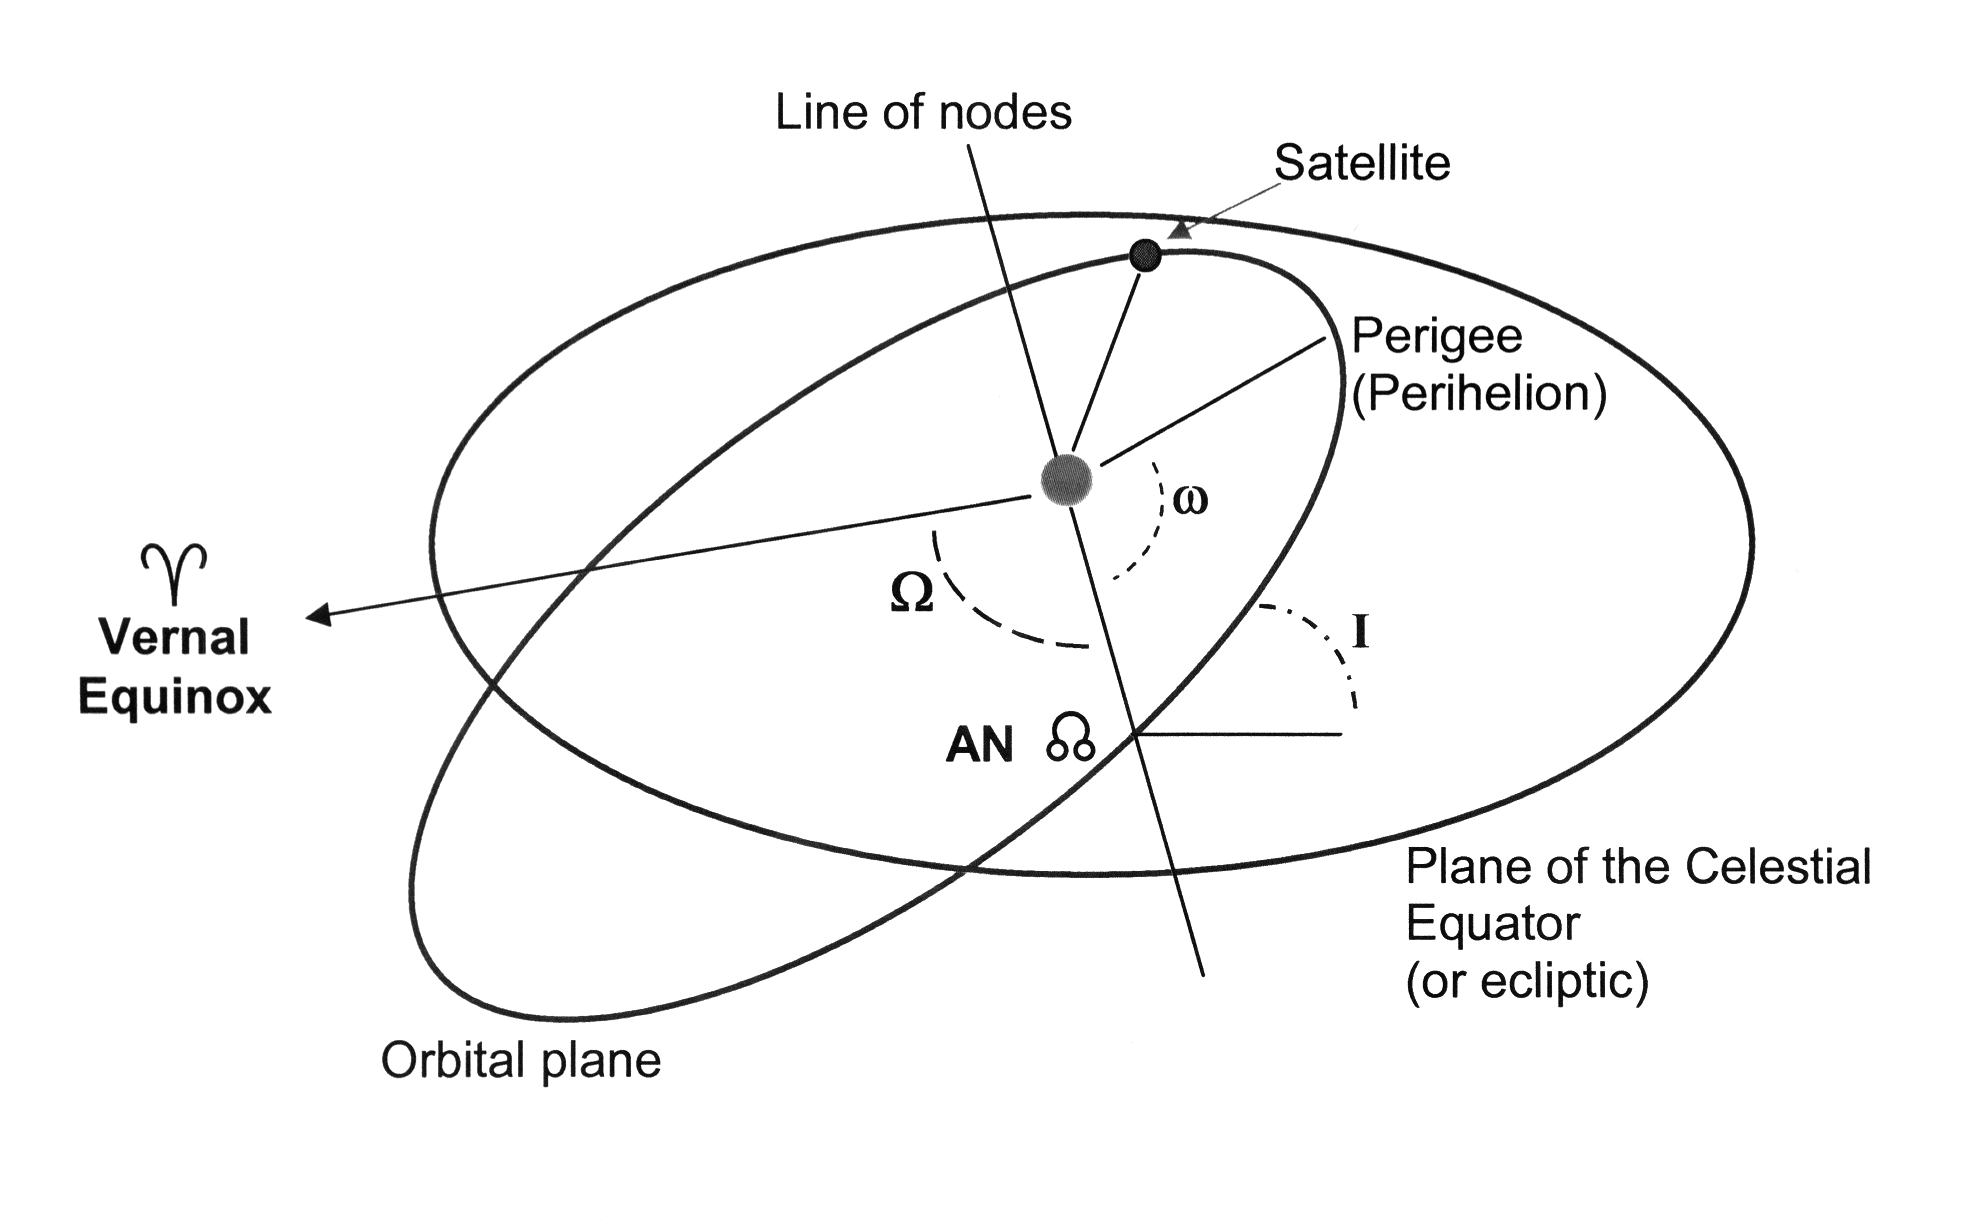
\includegraphics[scale=0.11]{orbitalparam.png}
\caption{Graphical representation of Keplerian Orbital Elements.}
\label{fig:orbitalparam}
\end{figure}


Each representation has pros and cons. Each of them can be used to identify uniquely the orbit in the space. The COE representation is often used for didactic purposes, but many models -- see \textit{Modeling the spacecraft maneuvers} -- use this because of it is more easy to make the computation. The TLE representation at the opposite: is shorter and more focused on trajectory prediction. The information is often updated many times in a day, during the crossing of a certain satellite over a tracking ground station.

From the site of Celestrack \cite{celestrack}, for each debris, has been extracted from the TLE and than, using the SPG4 software \cite{spg4}, the COE coordinates have been computed.



\subsection{Modeling the spacecraft maneuvers}
\begin{figure}[h]
\centering%
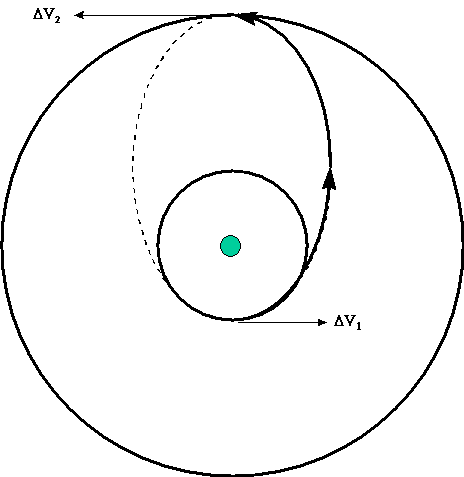
\includegraphics[width=5cm]{hohmann2.png}
\quad
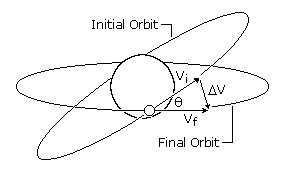
\includegraphics[width=5.5cm]{orbitalinclination.png}
\quad
\caption{Hohmann Trasfer in the same orbital plane (top) and inclination change manoeuvre (down).}
\label{fig:orbitalchange}
\end{figure} 
In order to remove a certain debris, the spacecraft needs to match the orbit of the objective. In real life, the debris removal needs to be performed by a rendezvous maneuver with the target but considering such a complex operation makes extremely complex the space of solutions. The assumption used in this project allows to model the transfer cost from a starting orbit to another, hence, the debris is considered removed if the spacecraft is matching its orbit.
The technique to reach the correct altitude is called \textbf{Three Impulse Manoeuvre}. It consists in three ignitions of the spacecraft's thrusters in three different points designed to minimize the amount of fuel expended. The first two are also known as \textbf{Hohmann Transfer Manoeuvre} -- Figure \ref{fig:orbitalchange} -- which objective is to transfer the probe from a lower orbit to a higher one. The first one is used to match the hight of the target orbit with the apoapsis - the highest point of an orbit. This orbit is also called Helliptical Transfert Orbit -- HTO -- because it transfers the spacecraft from the initial altitude to the objective one.
The next maneuver is done in the apoapsis of the HTO and it is used to circularize the Transfer Orbit to reach the periapsis altitude of the target orbit. Finally, the most expensive one is made in one of the two points in which the two orbits planes are crossing together: Ascending and Descending Node -- ANX and DNX. Figure \ref{fig:orbitalchange} shows their positions graphically. In the \textit{Appendix B}, the Python pseudocode shows how to compute the Three Impulse Manoeuvre to go from a starting orbit to the target one.



\subsection{How much dynamic is the problem}
The TSP is dynamic because the cities can't be considered fixed, such that their orbit is slowly changing during time due to the decay effect described in section \textit{Modeling the Environment}. Table \ref{tab:avgtransfcost} shows the distribution of the average transfer costs between city $i$ and city $j$ where $i \neq j$ at time $t_0$.

\begin{table}[h!]
\centering
\caption{Average transfer cost (m/s) at time $t_0$.}
\begin{tabular}{| l | c | c | c |}
\hline
     & \textbf{Iridium 33} & \textbf{Cosmos 2251} & \textbf{Fengyun 1C} \\ \hline
     mean & 5117.23  & 9095.58  & 8117.36  \\ \hline
     std  & 3906.69  & 4495.42  & 4883.83  \\ \hline
     min  & 10.86    & 38.29    & 25.23    \\ \hline
     25\% & 1937.61  & 5266.16  & 3482.05  \\ \hline
     50\% & 4177.21  & 9923.94  & 8367.70  \\ \hline
     75\% & 7484.08  & 13352.47 & 12859.28 \\ \hline
     max  & 15381.22 & 15160.57 & 16737.96 \\ \hline
\end{tabular}
\label{tab:avgtransfcost}
\end{table}

The Table \ref{tab:avgtransfcost} shows clearly that the standard deviation is very high, thus there are cities that could be extremely close one to the other, and others very far. 

In Table \ref{tab:avgdifftransfcost}, there is the average difference of the transfer costs between city $i$ and city $j$ where $i \neq j$, for each $t_i$ and $t_{i+1} \forall i \in V$. This table can give an immediate idea of the change of the cost for only a week. In particular, can be observed that Iridium33 and Cosmos2551 have more or less the same decay rate -- 9.62 -- such that all these debris belong to the same breakup events and are orbiting at the same high. The Fengyun 1C problem, due to the nature of its breakup \cite{nasahistory}, is characterized with sparser debris, therefore, the transfer cost between $i$ and $j$ may vary more than the other two sets.

\begin{table}[h]
\centering
\caption{Average difference of transfer costs (m/s) between time $t_i$ and $t_{i+1}$.}
\begin{tabular}{| l | c | c | c |}
\hline
 & \textbf{Iidium 33} & \textbf{Cosmos 2551} & \textbf{Fengyun 1C} \\ \hline
     mean & 9.63 & 9.62 & 42.09 \\ \hline
     std & 0.66 & 0.50 & 19.58 \\ \hline
     min & 7.30 & 7.82 & 8.79 \\ \hline
     25\% & 9.17 & 9.27 & 23.51 \\ \hline
     50\% & 9.61 & 9.62 & 43.08 \\ \hline
     75\% & 10.07 & 9.97 & 61.10 \\ \hline
     max & 12.47 & 12.04 & 76.42 \\ \hline
\end{tabular}
\label{tab:avgdifftransfcost}
\end{table}




%%%%%%%%%%%%%%%%%%%%%%%%%%%%%%%%%%%%%%%%%%%%%%%%%%%%%%%%%%%%%%%%%%%%%%%%%%%%%%%%

\section{Definition of the algorithm}
The Ant Colony Optimization \cite{ant1} -- ACO -- has been used to solve the DTSP. This algorithm is inspired by the natural behavior of the ant colony in nature. Those small animals, using pheromone tracks, are able to find food and adapt their behavior also in an environment that changes over time.
The ACO algorithm is a meta-heuristic. This means that it can be adapted for a wide number of problem. In order to solve the DTSP, the system is using a set of $K$ ants that have the objective of creating Hamiltonian cycles. It runs for a certain number of generations -- or iterations -- and the tour with the minimum cost is returned. In addition to the weight graph, the ants use a pheromone graph to store and spread the knowledge among all the ants and all the generation. This allows a form of cooperation that speeds up the search for the best solution. In addition to the cost measure, the ant uses the pheromone information as a measure of desirability for moving from the current city to the next one.
The following pseudo-code explain the ACO and the next subsections explain in details all the main functions:

\begin{lstlisting}[basicstyle=\scriptsize \ttfamily]
def ant_colony_optimization():
  pheromone_initialization()

  while generation < MAX_GENERATIONS:
    initialize_ant_position()
    state_transition_rule()
    pheromone_update()
	
  return best_solution
\end{lstlisting}

At the beginning of each generation, the ants are positioned randomly on the graph, and then create a Hamiltonian path using the state transition rule. In the next two subsections, the Pheromone management and the State Transition Rules are analyzed.


\subsection{Pheromone Initialization and Update}
As said before, the ants are sharing their knowledge laying a track of pheromone on the trail. This phenomena is called \textit{stigmergy} \cite{stigmergy}. The algorithm stores the pheromone in Pheromone Matrix $P$. The pheromone is initialized as:

\begin{equation}
\tau(i, j) := \frac{1}{(|V| \cdot nn_{cost}))}
\end{equation}

Where $nn_{cost}$ is the cost of the best solution found with the Nearest Neighbor Algorithm -- NN. Seen experimental results shown by \cite{izzo}, any rough approximation of the optimal tour length would work. The NN algorithm has been used to quick have the length estimation.

The Pheromone update is composed by two phases. The first one is the \textbf{Pheromone Evaporation}, while the second is the \textbf{Pheromone Allocation}. The first one is performed in order to avoid that the ants of the next generations continue to explore the same solution's space and also to allow exploitation for a shorter path. This evaporation is modeled as:

\begin{equation}
\tau(i, j) := (1 - \rho) \tau(i, j)
\end{equation}

Where $\rho$ is the evaporation rate. Than the \textbf{Pheromone Allocation} is performed \textbf{for each} of the $k$ tour produced by the current generation:

\begin{equation}
\tau(i, j) := \tau(i, j) + \frac{1}{cost(tour[k])}
\end{equation}


Such that the TSP is symmetric, also the Pheromone Matrix share this property. This means that for each of the previous formulas, the pheromone change is symmetrically propagated: $\tau(i, j) = \tau(j, i)$.

The complexity of the \textit{Pheromone Update} is $ O( \frac{n^2}{2} ) $ because the TSP is symmetric.


\subsection{State Transition Rule}
In order to create the Hamiltonian cycle, each ant has to choose the next city. The ACO algorithm uses a randomized constructive heuristic called State Transition Rule, that balance exploration and exploitation of the search space. At the beginning of each selection step, the exploration oriented \textbf{Random Proportional Rule} is selected with a probability less that $Q_0$, or the more exploitation-based \textbf{Pseudo-Random Proportional Rule} is used with probability of $(1-Q_0)$. The first one select the next city $s$ from the current city $r$ with a probability $p_k(r,s,t)$ at a certain time $t$:

\begin{equation}
p_k(r, s, t) = \frac{[\tau(r, s)^{\alpha}][\eta(r, s, t)^{\beta} ]}{ \sum_{ i \in J(k) }[\tau(r, i)^{\alpha}][\eta(r, i, t)^{\beta} ]}
\end{equation}

Where $J(k)$ is the list of available cities for the ant $k$, $\alpha$ is the importance of the pheromone trail and $\beta$ is the weight of heuristic information. For the last two, the greater they are, more likely the ant will use the information. Once computed all the probabilities for each available city belonging to $J(k)$, the exploration is performed selecting randomly the next city. 
The \textbf{Pseudo-Random Proportional Rule} is oriented on the exploitation and select the next city according to:

\begin{equation}
arg \;\; max_{u \in J(k)} { [\tau(i, j, t)^{\alpha}][\eta(i, j, t)^{\beta} ] }
\end{equation}

For each of the two rules $\eta(i, j, t) = 1 / \delta(i, j, t)$ were $\delta(i, j, t)$ is the distance between the city $i$ and $j$ at time $t$.
In \textbf{Appendix C} is listed the pseudocode of the State Transition Rule. The complexity of the \textit{State Transition Rule} is $O(n^2)$ for each ant $k$, where $n$ is the number of cities.

%%%%%%%%%%%%%%%%%%%%%%%%%%%%%%%%%%%%%%%%%%%%%%%%%%%%%%%%%%%%%%%%%%%%%%%%%%%%%%%%
\section{Population Based ACO: P-ACO}
Another popular variant in the ant systems is the Population-Based Ant Colony Optimization algorithm \cite{ant2}. As the name suggests, there is a population of solutions that maintain the knowledge of the previous iterations. This population has a fixed number of elements $\Phi$. At the end of each iteration, the best solution among the $K$ ants is selected and inserted. At the same time, a solution in the population is selected with some criteria, and then removed. There are different policies that can be applied:

\begin{itemize}
\item \textbf{Age}: the oldest ant is removed. The new solution is always inserted.
\item \textbf{Quality}: in the population there are only the best $\Phi$ solutions. Hence, is removed the worst one, if the new one has a better cost value.
\item \textbf{Prob}: \textbf{quality} tends to keep a lot of copies of the same solutions. In order to avoid that, the solution is removed with a probabilistic choice, using as weight the cost of each solution. The population to do the choice includes the new solution.
\item \textbf{Age and Prob}: as the name suggest it use the \textit{Age} for insertion -- the new solution is always inserted -- and the \textit{Prob} for the removal phase. The choice is done over the old solutions.
\item \textbf{Elitism}: one of the solutions -- usually the best of the population -- is selected and kept apart as Elite solution. It is is updated when a better solution is found. The Elitism can be applied to all of the previous techniques but it is especially useful for the Age Strategy to find the current best solution every iteration.
\end{itemize}


Obviously, for the first $\Phi$ iterations there will be the only insertion.
The main difference between the previous one -- ACO -- is that the update and evaporation of the pheromone are performed only when a new solution enters and exit from the population, as demonstrated by \cite{ant2}. For this work, the Age strategy without Elitism works better than the others four. The main reasons are that this strategy keeps high the diversity inside the population avoiding getting stacked in local minima \cite{ant2}. It is also the most efficient technique among all strategies, such that the population is implemented as a \textbf{circular array} of solutions. Maintaining the index of the first free position in the array, in which all operations are done, the final complexity results to be:

\begin{itemize}
\item \textbf{Insertion Cost} : $O(1)$
\item \textbf{Remove Cost} : $O(1)$
\end{itemize}

The \textbf{State Transition Rule} that selects the next city is kept as the ACO algorithm.
 
%%%%%%%%%%%%%%%%%%%%%%%%%%%%%%%%%%%%%%%%%%%%%%%%%%%%%%%%%%%%%%%%%%%%%%%%%%%%%%%%

\section{Local Search}
Two different local search methods have been selected in order to refine the solutions found by the best ants of each generation. The reason of using a local search is to increase the exploitation of the Ant Algorithms such that the search space changes every time a city is visited. 


\subsection{Non-deterministic 3 OPT}
One of the most famous local search algorithms is the 3-opt \cite{opt3}. It is based on the inversion of the sub-tour between two cities. Here, it is used a non-deterministic version in which the algorithm selects randomly six different indexes and then perform, one time, all possible inversions -- Figure \ref{fig:3optinverisions}. At the end of the procedure, the best solution is returned. The swap of a segment takes $O(1)$ such that the tour is implemented as a linked list. The most time-consuming phase is the computation of the tour cost, such that it must be done 7 times and costs $O(n)$ -- $n$ is the tour length -- each time. This leads the computation complexity to $ O( n ) $.

\begin{figure}[!h]
\centering
\captionsetup{justification=centering}
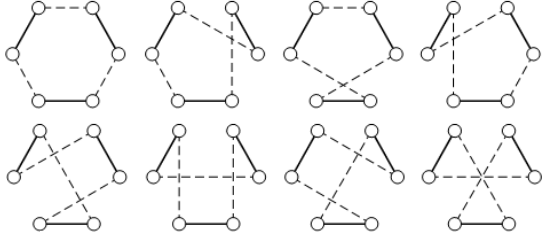
\includegraphics[width=7cm]{3opt.png}
\caption{List of all possible 3-opt inversions.}
\label{fig:3optinverisions}
\end{figure}



\subsection{Inver Over}
\begin{figure}[h]
\centering%
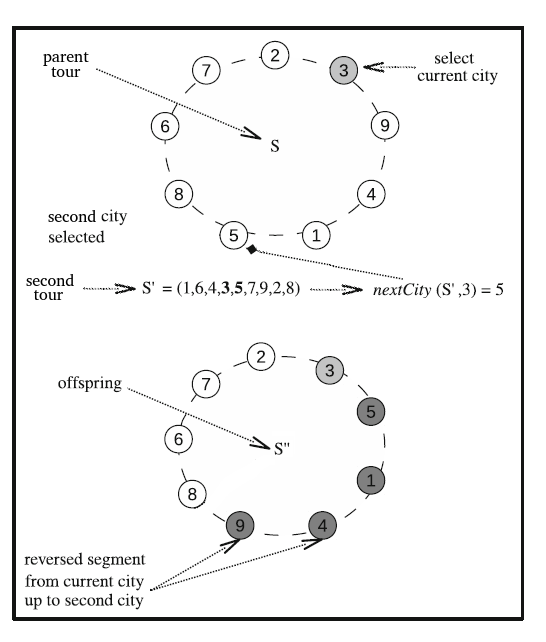
\includegraphics[width=7cm]{inverover.png}
\caption{Example of application of Inver-Over operator.}
\label{fig:inverover}
\end{figure}
In the field of local search, the Inver Over \cite{inverover} is an evolutionary technique widely used to solve the static TSP problem \cite{inverover_mica}. It is based on the inversion operator and it is applied to the best ant of every generation. The algorithm selects two different cities with some criterion, and reverse the path between the selected cities. The first city is randomly selected among those that belong to the best tour. The next one is selected from another solution. After a maximum amount of iterations (100), the algorithm is stopped and, if the solution has been improved, then it is updated. See Figure 4 for a graphical explanation of the algorithm.


%%%%%%%%%%%%%%%%%%%%%%%%%%%%%%%%%%%%%%%%%%%%%%%%%%%%%%%%%%%%%%%%%%%%%%%%%%%%%%%%

\section{Experimental results}
This section presents the experimental results. All of them, if not specified, are calculated with an average of 10 execution. The two ant algorithms are compared first against the Nearest Neighbours algorithm, and then among the different local search techniques: \texttt{normal} -- no local search applied --, \texttt{Non-determinitic 3-opt} and \texttt{io} -- Inver Over. All the tests were performed with a Windows 10 machine, with an Intel Core I7-7700 CPU - 2.80 GHz.
The parameters used for these tests are:

\begin{itemize}
\item $K$ = 5 : Number of ants.
\item $\alpha$ = 1 : Pheromone effect.  
\item $\beta$ = 6 : Heuristic effect.
\item $\rho$ = 0.9 : evaporation rate.
\item $Q_0$ =0.9 : Exploration / Exploitation Threshold
\item $Max\_Generations$ = 1000 : Max number of generations.
\item $\Phi$ -- Population Length: 100. Only for P-ACO.
\end{itemize}

\begin{figure}[!h]
\centering
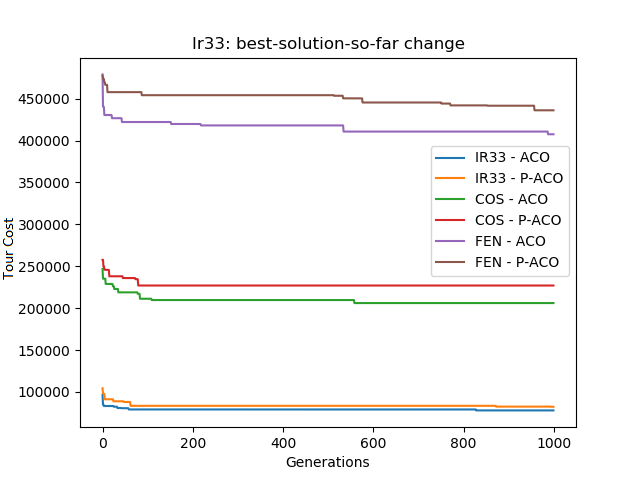
\includegraphics[width=8cm]{best_change.png}
\caption{Small example of change of the best solution cost among the generations.}
\label{fig:best_change}
\end{figure}

$Max\_Generations$ has been set to 1000 after some tests plotting the change of the best solution so far. See Figure \ref{fig:best_change} for an example of the change. As the plot shows, especially with large datasets, the solution is improved until the very end.

The first subsection -- \textit{Solution and Time Cost} -- faces the cost and the time expended to compute the results. The optimal solution for each dataset is not provided such that the dataset has been created for this project. Furthermore, there is not enough scientific interest in this topic, such that the debris problem is quite a new phenomena, nowadays faced only by national and international space agencies \cite{esadeb} \cite{nasadeb}.
The second subsection -- \textit{Local Search} -- shows the effectiveness of the two different local search approaches used.

\subsection{Solution and Time Cost}

\begin{table}[h!]
\caption{Average solution costs.}
\scriptsize
\renewcommand{\arraystretch}{1}
\begin{tabular}{|l|c|c|c|c|c|c|c|}
\hline
 \textbf{Cost} & \textbf{nn}        & \multicolumn{3}{c|}{\textbf{ACO}}          & \multicolumn{3}{c|}{\textbf{P-ACO}}         \\ \hline
     &        & \textbf{normal}    & \textbf{3-opt}     &  \textbf{io}      & \textbf{normal}    & \textbf{3-opt}     &  \textbf{io}      \\ \hline
\textbf{Ir33} & 86212  & \textbf{78007}  & 79444  & 78550  & 82310  & 78450  & 81897  \\ \hline
\textbf{Cos}  & 234550 & \textbf{205122} & 205502 & 205591 & 224810 & 224456 & 219168 \\ \hline
\textbf{Fen}  & 435408 & \textbf{407528} & 406921 & 416033 & 436117 & 434431 & 427408 \\ \hline
\end{tabular}

\label{tab:solcost}
\end{table}

The Table \ref{tab:solcost} shows that the ACO algorithm without any local search improvements seems to return the best solutions. Furthermore, the local search shows its effect only in the population-based version, in fact, the non-deterministic 3-opt get better results than the normal algorithm. The P-ACO algorithm seems not to perform very well for this problem, especially with large datasets.

The Table \ref{tab:soltime} compares the average time elapsed. It shows that that the local search has not a big impact on the system. This is because the search is performed only on the best ant of each generation.

\begin{table}[h!]
\caption{Average ellapsed time.}
\scriptsize
\begin{tabular}{|l|c|c|c|c|c|c|c|}
\hline
Time & nn    & \multicolumn{3}{c|}{ACO}  & \multicolumn{3}{c|}{P-ACO}         \\ \hline
     &       & normal & 3-opt  &  io    & normal & 3-opt  &  io      \\ \hline
Ir33 & 0.58  & 63.90  & 68.77  & 63.33   & 67.59  & 67.33  & 68.00  \\ \hline
Cos  & 6.56  & 200.57 & 218.05 & 234.66  & 207.36 & 206.10 & 232.98 \\ \hline
Fen  & 27.13 & 644.27 & 659.68 & 647.47  & 629.74 & 644.18 & 645.24 \\ \hline
\end{tabular}
\label{tab:soltime}
\end{table}

%%%%%%%%%%%%%%%%%%%%%%%%%%%%%%%%%%%%%%%%%%%%%%%%%%%%%%%%%%%%%%%%%%%%%%%%%%%%%%%%
\subsection{Local Search}
Table \ref{tab:numls} print out the average number of improvements performed by local search algorithms. These counters were increased only when the local search found a better solution. This measure can be seen as an indicator of the effectiveness of these approaches.
As the previous subsection explained, when an Ant algorithm is performing well, the number of local searches improvements is low. At the opposite, in the P-ACO case, the local search effect can be seen from the number of improvements performed, higher than in the ACO case.

\begin{table}[h]
\caption{Number of local search improvements.}
\scriptsize
\centering
\begin{tabular}{|l|c|c|c|c|}
\hline
     & \multicolumn{4}{c|}{ACO} \\ \hline
     &  \multicolumn{2}{c|}{3-opt} & \multicolumn{2}{c|}{io} \\ \hline
     & \textbf{Avg Increments} & \textbf{Agv Gain} & \textbf{Avg Increments} & \textbf{Avg Gain} \\ \hline  
Ir33 & 5.23   & 136.60 & 2.15 & 208.38   \\ \hline
Cos  & 2.28   & 152.98 & 0.67 & 152.98   \\ \hline
Fen  & 2.88   & 254.95 & 0.40 & 544.43   \\ \hline

\end{tabular}

\begin{tabular}{|l|c|c|c|c|}
\hline
     & \multicolumn{4}{c|}{P-ACO} \\ \hline
     & \multicolumn{2}{c|}{3-opt} & \multicolumn{2}{c|}{io} \\ \hline
     & \textbf{Avg Increments} & \textbf{Agv Gain} & \textbf{Avg Increments} & \textbf{Avg Gain} \\ \hline  
Ir33 & 57.61  & 77.86  & 225.59 & 105.61  \\ \hline
Cos  & 38.46  & 90.71  & 162.11 & 127.04 \\ \hline
Fen  & 39.26  & 89.24  & 151.59 & 184.86 \\ \hline
\end{tabular}
\label{tab:numls}
\end{table}

%%%%%%%%%%%%%%%%%%%%%%%%%%%%%%%%%%%%%%%%%%%%%%%%%%%%%%%%%%%%%%%%%%%%%%%%%%%%%%%%
\subsection{Solution's Diversity}
A possible problem that could affect the Ant algorithm effectiveness is the lack of diversity among the solutions. Keeping high this parameter is very important, such that, from the old solutions, the pheromone matrix is updated and the future ants will base their search. A lack of diversity means being stuck in a local minimum. For this reason, a diversity measure has been computed on all the set of feasible solutions $S$, created during all the iterations of the algorithm -- generations. It is defined as:

\begin{equation}
Div = \frac{\sum_{i \in S}\sum_{j \in S, j \neq i}^{|S|} CE(i, j)}{|S|(|S| - 1)}
\end{equation}

Where:

\begin{equation}
CE(i, j) = 1 - \frac{\#~common~edges}{\#~edges}
\end{equation}

If all the solutions are different, the diversity will be 1.0. At the opposite, if all the solutions are equal, it will be 0.0. For both of the algorithms (in all cases) the diversity is very high: the average is 0.98, with a standard deviation of 0.0036. This aspect proves that the Ant colony algorithms have a superb capability in avoiding local minimum.

 

%%%%%%%%%%%%%%%%%%%%%%%%%%%%%%%%%%%%%%%%%%%%%%%%%%%%%%%%%%%%%%%%%%%%%%%%%%%%%%%%
\section{Conclusion and further research}
The classical Ant Colony Optimization algorithm proved that it is capable of solving the Dynamic TSP. Meanwhile, the Population-Based ACO showed poor results and generally a lack of exploitation. Also, the local search showed no great impact on the final results, especially when the algorithm is performing well. 

Future researches should focus on the long-term forecast of the orbital debris decay model.
One of the strongest simplifications that have been used in this project was the assumption that when the spacecraft get an orbit, it instantaneously removes a debris. This problem should be solved from two points of view. The first is to include the removing time in the model, while the second is to model the more realistic rendezvous maneuver, although it will drastically increase the complexity of the data generation.

A step in this direction could be to allow the spacecraft to wait for a more favorable environment. Therefore it could choose to keep the same orbit for more than $t_i$. This obviously leads to having $|T|$  $|V|$.
Another important aspect to tackle is the application of new local search algorithms, in order to put more effort into the exploitation of the solutions. More effort must be put on the automatic adaptiveness of all the numerous parameters of the algorithm, that in this project have been tuned manually.


%%%%%%%%%%%%%%%%%%%%%%%%%%%%%%%%%%%%%%%%%%%%%%%%%%%%%%%%%%%%%%%%%%%%%%%%%%%%%%%%

\section{Appendix A}
Here there is the python pseudocode that for each debris can compute the loss in the orbital period due to the drag. The algorithm is developed by \cite{australia}. For each debris the procedure needs:
\begin{itemize}
\item \textbf{RE} : $ 6378137 $ : Radius of the Earth in meters.
\item \textbf{periapsis\_height} : height of the periapsis in meters.
\item \textbf{WEEK} : A week in seconds. The algorithm predict the loss of period time after a week of simulation.
\item \textbf{MU} :  $3.983324e14$ : Earth Gravitational Constant.
\item \textbf{f10\_param} : Flux 10 parameter of the solar wind \cite{f10flux}.
\item \textbf{ap\_param} : Geomagnetic index \cite{ap}. 
\item \textbf{A} : Area of the debris \cite{act}.
\item \textbf{m0} : Mass of the debris \cite{act}.
\item \textbf{Cd} : Drag coefficient. It depends from the orbit hight. $ 2.1 <= Cd(h) <= 2.4 $ 
\end{itemize}


\begin{lstlisting}[basicstyle=\scriptsize \ttfamily]
def compute_orbital_decay():
  # Compute orbital decay from the periapsis height.
  # The step is one week.
  h = (periapsis_height - RE) / 1000

  r = RE + h * 1000
  # initial Period.
  P = [2 * pi * sqrt(pow(r, 3) / MU)]
  t = [0]

  dt = WEEK  # a week in seconds

  # Below 181 Km is considered as removed.
  while (h >= 181):
    # retrieve the solar flux elements.
    f10_param = retrieve_flux()
    # retrieve the geomagnetic elements.
    ap_param = retrieve_ap()

    sh = (900 + 2.5*(f10_param[h] - 70)
         + 1.5*ap_param[h]) 
         / (27 - 0.012*(h - 200))
            
    # Cd is the drag hight coefficient.
    dP = 3*pi*A*Cd(h) / m0*r*dt*exp(-(h - 175) / sh)
    dP = dP * 6e-10
   
    P.append(P[-1] - dP) # decrement in orbital period
    t.append(t[-1] + dt) # compute new time value
    
    # new orbital radius
    r = pow(MU*(pow(p[-1], 2) / 4*pi*pi), 0.3333) 

    h = (r - RE) / 1000 # new altitude (semimajor axis)

  return P
\end{lstlisting}

\section{Appendix B}
In this appendix there is the code for computing the Three Impulse Manoeuvre.

\begin{lstlisting}[basicstyle=\scriptsize \ttfamily]
def manouver(str_orbit, fnl_orbit):
  # First manoeuvre: Hohmann Transfer
  a = (str_orbit.periapsis + fnl_orbit.apoapsis) / 2
  tngt_velocity = sqrt(MU * (2 / fnl_orbit.apoapsis - 1 / a))
  delta_1 = abs(tngt_velocity - str_orbit.vel_periaps)

  # Second manoeuvre: circularization
  delta_2 = abs(tngt_velocity - fnl_orbit.vel_apoapsis)
 
  # inclination change:
  cos_delta_i = cos(str_orbit.incln) * cos(fnl_orbit.incln)
    + sin(str_orbit.incln) * sin(fnl_orbit.incln) 
    * cos(str_orbit.raan) * cos(fnl_orbit.raan)
    + sin(str_orbit.incln) * sin(fnl_orbit.incln)
    * sin(str_orbit.raan) * sin(str_orbit.raan)
    
  delta_i = sqrt(pow(fnl_orbit.vel_apoapsis, 2) 
    + pow(fnl_orbit.vel_periaps, 2)
    - 2 * fnl_orbit.v_a * fnl_orbit.vel_periaps * cos_delta_i)
  
  return delta_1 + delta_2 + delta_i
\end{lstlisting}

\section{Appendix C}
Appendix C exposes the State Transition Rule in Python pseudo-code. For each ant $k$, the function creates a tour choosing the next cities according to the Random Proportional Rule or the Pseudo Random Proportional Rule. $available$ is a list of the sets (one for each ant) of the unvisited cities.

\begin{lstlisting}[basicstyle=\scriptsize \ttfamily]
def state_transition_rule():
  """For each ant k, choose the next city."""
  for k in range(N_ANTS):     
    t = 0 # time iterator.
    for i in range(N_CITIES - 1):
      # get the current city.
      r = self.tours[k][-1]

      # pick a random number.
      rnd_n = random()
      if rnd_n < Q0:
        next_city = rnd_prop_rule(r, available[k])
      else:
        next_city = pseudo_rnd_prop_rule(r, available[k])
		
      # remove the city just visited from the availables.
      available[k].remove(next_city)  
        
      # append the new city to the tour.
      tours[k].append(next_city)
		
      # increment the time iterator.        
      t = t + 1

\end{lstlisting}

%%%%%%%%%%%%%%%%%%%%%%%%%%%%%%%%%%%%%%%%%%%%%%%%%%%%%%%%%%%%%%%%%%%%%%%%%%%%%%%%


\begin{thebibliography}{9}
\bibitem{kessler}
D. J. Kessler, B. G. Cour-Palais.
\textit{Collision frequency of artificial satellites: The creation of a debris belt.}
Journal of Geophysical Research: Apace Physics. (1978-2012), 83(A6):2637-2646, 1978.

\bibitem{cam}
H. Krag, K. Merz, T. Flohrer, S. Lemmens, B. Bastida Virgili, Q. Funke, V. Braun.
\textit{ESA’s Modernised Collision Avoidance Service.}
14th International Conference on Space Operations (2016).

\bibitem{esatech}
K. Wormnes, R. Le Letty, L. Summerer, R. Schonenborg, O. Dubois-Matra, E. Luraschi, A. Cropp, H. Krag, J. Delaval.
\textit{ESA Technologies for Space Debris Remediation}
6th European Conference on Space Debris. Vol. 1. ESTEC, Noordwijk, The Netherlands: ESA Communications, 2013.

\bibitem{leo}
J. C. Liou, N. L. Johnson.
\textit{Instability of teh present leo satellite populations.}
Advances in Space Research, 41(7):1046-1053, 2008.

\bibitem{izzo}
Dario Izzo, Ingmar Getzner, Daniel Hennes, Luís F. Simões.
\textit{Evolving solutions to TSP variants for active space debris
removal.}
GECCO'15 Conference, July 11 2015, Madrid, Spain. 2015.

\bibitem{adr_tsp1}
B. W. Barbee, S. Alfano, E. Piñon, K. Gold, D. Gaylor.
\textit{Design of Spacecraft Missions to Remove Multiple Orbital Debris Object.}
35th Annual AAS Guidance and Control Conference. 2012.

\bibitem{adr_tsp2}
M. Cerf.
\textit{Multiple Space Debris Collecting Mission: Debris Selection and Trajectory Optimization.}
Technical Report. EADS Astrium Space Transportation. 2012.

\bibitem{china}
T.S. Kelso.
\textit{Analysis of the 2007 Chinese ASAT Test and the Impact of its Debris on the Space Environment.}
AMOS Conference. Technical Paper. Maui, Hawaii. 2007.

\bibitem{celestrack}
T.S. Kelso.
\textit{https://celestrak.com/}
Website held by Center for Space Standards and Innovations (CSSI).

\bibitem{trafficjam}
C. J. Eycklhof, M. Snoek.
\textit{Ant Systems for a Dynamic TSP Ants caught in a traffic jam.}
International Workshop on Ant Algorithms ANTS 2002: Ant Algorithms pp 88-99, 2002.

\bibitem{pheromod}
M. Guntsch, M. Middendorf.
\textit{Pheromone Modification Strategies for Ant Algorithms Applied to Dynamic TSP.}
E.J.W. Boers et al. (Eds.) EvoWorkshop 2001, LNCS 2037, pp. 213–222, 2001.

\bibitem{immigrants}
M. Mavrovouniotis, S. Yang.
\textit{Ant colony optimization with immigrants schemes for the dynamic travelling salesman problem with traffic factors.}
Applied Soft Computing 13, 4023–4037. 2013.

\bibitem{spg4}
David A. Vallado, Paul Crawford.
\textit{SGP4 Orbit Determination.}
American Institute of Aeronautics and Astronautics.

\bibitem{act}
Advanced Concept Team. European Space Agency.
\textit{http://www.esa.int/gsp/ACT/mad/projects/debris\_removal.html}
Website of the Advanced Concept Team regarding the debris removal datasets.

\bibitem{australia}
John Kennewell.
\textit{Satellite Orbital Decay Calculations.}
Ips Radio and Space Services. The Australian Space Weather Agency.

\bibitem{f10flux}
K. F. Tapping.
\textit{The 10.7 cm solar radio flux.}
Space Weather, Vol. 11. 394 - 406, doi:10.1002/swe.20064, 2013. 

\bibitem{ap}
H. S. Ahluwailia.
\textit{The predicted size of cycle 23 based on the inferred three-cycle quasi-periodicity of the planetary index Ap.}
Journal of Geophysical Research, Vol. 103, NO. A6, Pages 12,103-12,109, June 1, 1998.

\bibitem{nasahistory}
N. Johnson, E. Stansbery, D. Whitlock, K. Abercromby, D. Shoots.
\textit{History of On-Orbit Satellite Fragmentations.}
Orbital Debris Program Office. Technical Report. NASA/TM-2008-214779, S-1030. May 01, 2008.

\bibitem{ant1}
M. Dorigo, L. M. Gambardella.
\textit{Ant Colony System: A Cooperative learning approach to the Travelling Salesman Problem.}
IEEE Transaction on Evolutionary Computation, Vol. 1, No. 1. April 1997.

\bibitem{stigmergy}
J. L. Deneubourg.
\textit{Application de l'ordre par fluctuations á la description de certaines étapes de la construction du nid chez les ternutes.}
Insect Sociaux, Vol 24, pp 117-130, 1977.

\bibitem{ant2}
M. Guntsch, M. Middendorf.
\textit{Applying Population Based ACO to Dynamic Optimization Problems.}
Ants 2002, LNCS 2463. pp 111-122, 2002.

\bibitem{opt3}
K. Helsgaun.
\textit{An effective implementation of the Lin-Kernighan travelling salesman heuristic.}
European Journal of Operational Research 126 106-130. 2000.

\bibitem{opt32}
A. Blazinskas, A. Misevicius.
\textit{Combining 2-OPT, 3-OPT and 4-OPT with K-Swap-Kick perturbations for the travelling salesman problem.}
Kaunas University of Technology, Department of Multimedia Engineering, Studentu St. 50-401, 416a, Kaunas, Lithuania. 

\bibitem{inverover}
M. Mavrovouniotis, S. Yang.
\textit{A memetic ant colony optimization algorithm for the dynamic travelling salesman problem.}
Soft Computing 15:1405–1425. 2011.

\bibitem{inverover_mica}
T. Guo, Z. Michalewicz.
\textit{Inver-over operator for the TSP.}
Proceedings of the 5th international conference on parallel problem solving from nature. pp 803–812. 1998

\bibitem{esadeb}
Space Debris Office. European Space Agency.
\textit{https://www.esa.int/Our\_Activities/Operations/Space\_Debris}

\bibitem{nasadeb}
Orbital Debris Program Office. NASA.
\textit{https://www.orbitaldebris.jsc.nasa.gov/}

\end{thebibliography}

\bibliography{Mendeley}
%%%%%%%%%%%%%%%%%%%%%%%%%%%%%%%%%%%%%%%%%%%%%%%%%%%%%%%%%%%%%%%%%%%%%%%%%%%%%%%%
% biography section


%%%%%%%%%%%%%%%%%%%%%%%%%%%%%%%%%%%%%%%%%%%%%%%%%%%%%%%%%%%%%%%%%%%%%%%%%%%%%%%%
\newpage
\onecolumn
\end{document}